\documentclass[extra,mreferee]{gji}
%\usepackage{timet}

\usepackage{graphicx}
\graphicspath{ {./figures} }
\usepackage{subfig}
\usepackage{caption}
\usepackage{floatrow}
\usepackage{amssymb}
\usepackage{commath}
\usepackage{amsmath}
\usepackage[dvipsnames]{xcolor}
\floatsetup[figure]{style=plain,subcapbesideposition=top}
%\usepackage[margin=70mm]{geometry}

%\usepackage{subfig}

\title[\texttt{gji\_extra.sty} ]
  {\texttt{GLAD-M25} - global adjoint tomography model}

\author[]  {Wenjie lei, Jeroen Tromp, ...}

\newcommand{\btx}{\textsc{BibTeX}}

\begin{document}

\maketitle

\section{Introduction}
With the development of high performance computing and numerical methods, it is now possible to using adjoint method to image the interior the globe using thousands of earthquakes.

There are few agreements about the earth model and yet many unknown to be resolved. There are quite a lot of global models exits however there is no such con-sense.

The GLAD-M25 is the first earth model that incorporate the P and S wave speed using full waveform inversion. Also, people are using specific set of phases in their inversion. For P models, people are using P phase and other body wave phases and for S models, people are using mostly S wave phases and surface waves to constrain the structure. Those two kinds of models usually reveals very different parts of the earth. For example, for P wave, people used it the image the subduction slabs and it is not very good at image lower mantle structures, such as plumes and lower mantle convection. For S waves, it is the verse verso.

There are many challenges coming along the way. First, the data volume is huge.  There are in total of 1480 earthquakes used in the inversion stage, added into the database step by step. Second, workflow management is crucial dealing with such a large project. One factor is coming from the complex workflow. There are 4 major building blocks, forward simulation, seismic data processing, adjoint simulation and post-processing. Each blocks contains several small blocks. The other factor is coming from the number of earthquakes and high demands of computation. In each iteration, we are doing 1480 forward and adjoint simulation, generating a few Petabytes of wavefield files and consuming 16 million of CPU hours on the supercomputer at Oak Ridge National Lab. There are yet more in data processing stages. How to deal with hardware failures is very important and prevent contamination into our inversion results.

Here, we present our GLAD-M25 earth model, with significantly improvements on the plumes and subductions.

test1 (\cite{zhu2012structure}, \cite{zhu2012structure})
test2 \citep{zhu2015seismic, ekstrom2012global}
test3 \citet{ekstrom2012global}


\section{Starting Model GLAD--M15}

As the continuation of our previous work, we used GLAD-M15 as our
starting model\citep{bozdaug2016global}.
The GLAD-M15 is a 3D transversely isotropic earth model. Its uses
GLAD-M00, a combined 3-D mantle model S362ANI \citep{kustowski2008anisotropic}
with 3-D crust model CRUST2.0 \citep{bassin2000current}, as its own starting model.
Instead of relying to the "crust correction", SPECFEM mesher enables us to incorporate
the 3D crustal model so we are able to update the crust and mantle structures at same
time with any trade-off. Besides, the.

GLAD-M15, same as  S362ANI, provides 6 model parameters, mass density($\rho$), two compressional
wavespeeds($\alpha_v$ and $\alpha_h$), two shear wavespeeds($\beta_v$
and $\beta_h$) and a dimenionless parameter($\eta$). We will discuss
the model parametrization in detail in the following sections.

GLAD-M15 then uses 256 earthquakes and broad-band seismic data to do the 3D full-waveform
inversion\citep{bozdaug2016global}. The first 12 iterations of GLAD-M15 was
performed under 27 secs and the last 3 under 17 secs. We will keep our model
resolution as 17s in our model. As shown in our later analysis,
GLAD-M15 proven good enough improvements over S362ANI in both our inversion
dataset and held-out test dataset. It also shows both significant misfit reduction
in all measurement categories and and better behavior in statistic analysis from distribution
of the phase measurements, which will discussed in the following sections.

\section{Earthquakes}
In addition to the 256 earthquakes used in the first generation model GLAD-M15, we
carefully picked 784 more earthquakes from Global Centroid-Moment-Tensor catalog\citep{}
and added them into our database, making the total number of earthquakes reach 1,040.
The lower band of moment magnitude, is set at 5.5 to ensure the signal-to-noise ratio at
the global scale. The upper bound of magnitude is set at 7.2 and duration of earthquakes
is set at 9 sec since we can use point representation and Gaussian-type source
time function.
We also constrain the duration of CMT sources to be smaller than 17s.
The locations of 1040 earthquakes is shown in fig.\ref{fig:source_correction}a.

To ensure a even global coverage, we used the seismic stations mainly from several global
seismic networks such as Global Seismic Network(II, IU, IC, US, CU and GT),
GEOFON(GE), GEOSCOPE(G), and regional networks, such as MedNet(MN),
, Brazilian Lithospheric Seismic Project(BL), Chilean National Seismic Network(C), Japan Meteorological
Agency Seismic Network(JP) and etc. The number of seismic stations usually ranges
from 150 to 500, depending on the availability of seismic stations when the earthquake
happened. The distribution of seismic stations is in Fig.\ref{fig:source_correction}b and
data is download from the Incorporated Research Institutions for Seismology(IRIS).

We use the source inversion algorithm of \cite{liu2004spectral}. This algorithm set the
target misfit function as the normalized waveform difference and envelope difference between
observed data, \textbf{d} and synthetic data generated from GLAD-M15, \textbf{s}.

\begin{multline}
  \chi = \sum\limits_{c=1}^{N_c} \omega_c \sum\limits_{r=1}^{N_r} \omega_{cr}
       \sum\limits_{m=1}^{N_m} \omega_{crm}
       \Big\{ \lambda {\frac
              { \int \big[ \mathbf{d}_m(t) - \mathbf{s}_m(t - \Delta t, \mathbf{m}_{15}) \big]^2 dt }
              {\int \big[ \mathbf{d}_m(t) \big]^2  dt } }\\
         + (1 - \lambda) \frac
              {\int \big[ e(\mathbf{d}_m(t)) - e(\mathbf{s}_m(t - \Delta t, \mathbf{m}_{15})) \big]^2 dt }
              {\int \big[ e(\mathbf{d}_m(t)) \big]^2  dt} \Big\}
\end{multline}

Following \cite{ekstrom2012global}, seismograms were filtered into 50-100s
to select 3-component body wave windows and 60-100s to select 3-component
surface wave windows. Thus, the number of measurements categories $N_c$,
is 6. To balance the contribution from each category, the weighting for each
category $\omega_c$, is the reciprocal of the number of measurements in that
category. The $N_r$ is the number of seismic stations in one category. $\omega_r$
is the receiver weighting assigned to each individual stations, which we will discuss
that in detail in the following sections. $N_m$ is the number of measurements for one
seismic stations in one measurements category and $\omega_m$ is the measurements weightings
, which is simply set to 1. The inverted parameters includes moment tensors, longitude,
latitude and depth. In order to get the frechet derivatives for each parameter, there is
one global-scale forward simulation needed to be done so the source inversion becomes a very expensive
operation.

Since we shifted the synthetic data based on the cross-correlation to its correspond observed
data to the best match of the pair, our source inversion is not very sensitive to
the origin time of earthquakes. In addition to prepare the future Q inversion,
A grid search for the origin time and scalar moment correction was introduced
directly to future calibrate the sources afterwards following \cite{zhu2012structure}.
The grid-search calibration has a linear effect on the seismograms so it doesn't take extra
simulation time.

Fig.\ref{fig:source_correction} shows the source correction results.
Most of the earthquakes shows a shallower depth after the source inversion
(Fig.\ref{fig:source_correction}b and Fig.\ref{fig:source_correction}c),
in consistent with \cite{hjorleifsdottir2010effects}.
We observed $-2.62\pm2.49$km depth change compared with the global CMT solutions.
The scalar moment, on the average, has $5.31\pm3.91$\% change and change of origin time
is $-0.60\pm1.17$ sec.

Starting from GLAD-M22, we added extra 440 earthquakes from GLobal CMT catalog,
mainly in previously poorly covered regions. However, due to computational cost,
we didn't implement the 1st stage source inversion in the newly added 440
earthquakes but only calibrate its origin time and scalar moment.

\begin{figure}
  \centering
  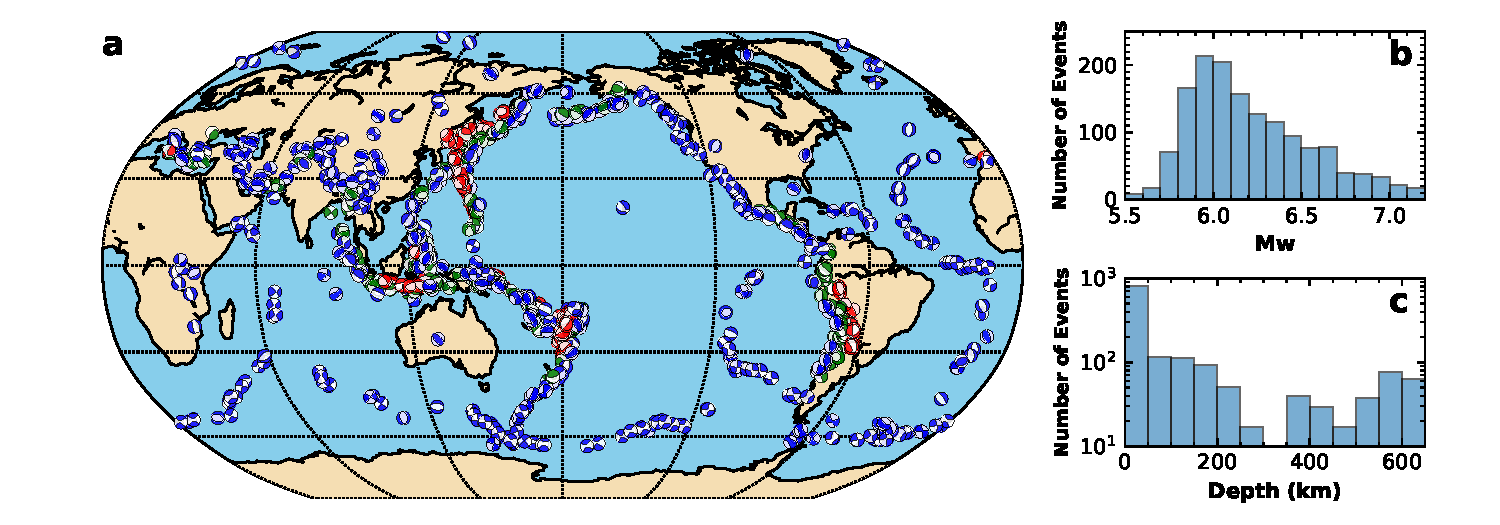
\includegraphics[width=\textwidth]{figures/events_1480.pdf}
  \caption{1480 earthquakes used in this study. (a) Distribution of earthquakes. Colors of beach balls indicate the depth range of earthquakes from Global CMT Catalog \citep{ekstrom2012global}. {\textbf{\color{Blue} Blue}} is for shallow earthquakes above 50km, \textbf{{\color{ForestGreen} Green}} is between 50 and 300km and \textbf{{\color{Red} Red}} is below 300km. (b) and (c) Histograms of earthquake moment magnitudes and depths.}
  \label{fig:event_1480}
\end{figure}

\begin{figure}
  \centering
  \includegraphics[width=\textwidth]{figures/source_corrections.pdf}
  \caption{Source correction results for 1040 events used in the inversion. (a) Map views of depth changes. (b) Distribution of seismographic stations used in the source inversion stage.(c) depth change of CMT sources compared to its initial solution from the Global CMT Catalog. (d)-(f) Histograms of depth, origin time and scalar moment changes.}
  \label{fig:source_correction}
\end{figure}

\section{Seismic Data}

Seismic stations have been very carefully picked to ensure global coverage and high data quality.
Other than the networks we mentioned in the source inversion, we include all the data we can
downloaded from IRIS data center. Regional and temporary networks has become a significant part
in our database and greatly improve the ray coverage at specific regions, such as US Array(TA),
Africa Array(AF), Canadian National Seismograph Network (CN), Geoscience Australia (AU),
Brazilian Lithospheric Seismic Project (BL),
Antarctic Seismographic Argentinean Italian Network (AI),
the New Zealand National Seismograph Network (NZ) and etc.

The data, associated with the earthquakes, was downloaded from several data centers,
including IRIS, ORFEUS, INGV, IPGP, ETH, GEONET and etc.
There are in total of 275 seismic networks (with individual network code) and 11,800
seismic stations used in the structural inversion stage. Fig.\ref{fig:stations}
shows the distribution of seismic stations.

\begin{figure}
  \includegraphics[width=0.8\textwidth]{figures/station_map.pdf}
  \caption{Distribution of 11,800 seismographic stations on the globe. Colors denote the number of events which they contribute waveforms to in the model inversion stage. Stations with event response < 400 are plotted in smaller size and they are usually temporary arrays which are deployed over a short period of time. The max event reponse comes from IU.ANMO, which contributeed to 1442 out of 1480 eartquakes in out dataset.}
  \label{fig:stations}
  \centering
\end{figure}

\section{Misfit function and Model Parametrization}

This sections will discuss how we define the the misfit function and how we parameterize the model.
The overall misfit, $\Phi$, is defined as follows:

\begin{align}
\label{eq:misfit}
\Phi = \sum_{s}^{S} \omega_s \sum_{c}^{C} \omega_{c} \sum_{r}^{R_{sc}} \omega_{scr} \sum_{w}^{N_{scr}} \omega_{scrw}\, \chi_{scrw}
\quad ,
\end{align}\\
where~$S$ denotes the number of sources, $C$ the number of categories,
$R_{sc}$ the number of receivers for source~$s$ and category~$c$,
and~$N_{scr}$ the number of measurements for source~$s$, category~$c$
and receiver~$r$.

The misfit for source~$s$, category~$c$, receiver~$r$, and window~$w$ is
\begin{align}
  \chi_{scrw} = \int \Big[ \frac {\Delta \tau_{scrw}} {\sigma_{scrw}} \Big]^2 d\omega
\quad ,
\end{align}
is a frequency-dependent phase measurements using then multitaper technique.
where $\Delta m_{scrw}$ denotes a measurement with associated standard deviation~$\sigma_{scrw}$.-

\subsection{Weightings}
Weighting is crucial to the global tomography to compensate the uneven distribution
of earthquakes and seismic stations. First, most of the earthquakes happen in the
in the plate boundaries. There are also several seismic active zones, such as Japan,
Fiji Tonga and South America, where there are a lot of earthquakes clustered near
the subduction slabs.
Second, most of the seismic stations located in the continents, especially located in
the northern hemisphere. Besides, there are quite a few dense seismic arrays,
for example US array, deployed recently, which has hundred or thousands of instrument deployed
at the regional scale, which will has a very strong footprint on the misfit gradients if no weighting
been applied.

All the factors mentioned above will lead to a uneven distribution of
ray paths and thus uneven sampling of the earth structure. Our weighting strategy
is developed to compensate such effects. There are two terms in the misfit function
receiver weightings, $\omega_{scr}$, and source weightings $\omega_{s}$.
The calculation of both terms can be abstracted as: given the distribution of
points determine the weighting associated with each point.
Here we introduce the exponential weightings to describe the density of points and
determine the point weightings. Given a set of points $p_i$, the distance between
two is $r_{ij}$, the weightings associated with each point, $w_i$, could be obtained by:

\begin{equation}
w_{i} = \frac{1}{A} \left(
  \sum_{j=1}^N \exp \left[ \mbox{} - \left( \frac{r_{ij}} {r_{0}} \right)^2 \right] \right) ^{-1}
\label{eq:spatial_weights}
\end{equation}
where $r_{0}$ is the sensitivity distance and $A$ is the normalization term.
The reference distance $r_0$ will control ratios of weightings between dense and
sparse regions. For more details for the weightings, please refer to the Appendix XXX.

\subsection{Model Parametrization}
Transversely isotropy model parametrization is used in our model, same as S362ANI(GLAD-M00)
and GLAD-M15. Comparing to a general anisotropic model which has 21 independent variables,
our model could be described by 5 Love parameters, A, C, L, N and F\citep{love2013treatise}.
Since it is more straight forward to use  wavespeed as model parameters in sesimology,
we choose $\alpha_v$, $\alpha_h$, $\beta_v$, $\beta_h$ and $\eta$.
Assuming the radial anisotropy is due to shear anisotropy, these 5 parameters
can be further reduced to 4, we introduced the bulk sound speed,
$c=\sqrt{\kappa/\rho}$. Our final parameters are:\\
\begin{align*}
      c &= \sqrt{\kappa/\rho} \\
\beta_v &= \sqrt{L/\rho} \\
\beta_h &= \sqrt{N/\rho} \\
\eta & = F/(A-2L)
\end{align*}

Since density is hard to constrain due to the period band we are working on, the $\rho$ kernel is obtained by scaling the isotropic shear wavespeed kernel\citep{montagner1989petrological},\\
\begin{equation*}
    \delta ln\rho = 0.33\delta ln\beta
\end{equation*}

where $\beta$ is defined as the Voigt average of the raidally anisotropic shear wave speeds\citep{babuska1991seismic}
$$\beta = \sqrt{(2\beta_v^2 + \beta_h)/3}$$

Based on the parametrization described above, the perturbations in misfit functions would be:

\begin{equation*}
    \delta \chi = \int_V
      (K_c\delta lnc + K_{\beta_v}\delta ln\beta_v + K_{\beta_h}\delta ln\beta_h +
      K_\eta \delta ln\eta) dV
\end{equation*}

\section{Adjoint Tomography Workflow}

The flow chart for adjoint tomography is shown in Fig.\ref{fig:adjoint_workflow}.
The workflow starts with a certain number of earthquakes. Here, we used the
inverted CMT sources from the Global CMT catalog. Based on the time
of earthquakes, we downloaded observed data, including time series and StaionXML,
from IRIS and other data centers. The we convert the sources, StationXML and time series
into ASDF files. Each ASDF file usually contains a complete set of data from one
earthquake. The data download and conversion need to be done only once. The raw observed data,
storing in ASDF, could be reused afterwards.

\begin{figure}
  \centering
  \includegraphics[width=\textwidth]{figures/adjoint_workflow_6.pdf}
  \caption{Adjoint Tomography Workflow.}
  \label{fig:adjoint_workflow}
\end{figure}

\subsection{Forward simulation}
The forward simulation takes the CMT sources, stations and Earth models as input.
We will first generate mesh based on the models. The CMT sources and station will
be fed into the solver to generate synthetic seismograms and forward wavefield snapshots.
SEPCFEM3D\_GLOBE with GPU acceleration is used on Titan at the Oak Ridge Nation Lab for
both mesher and solver part.

To simulate 120min of seismograms at 17sec resolution, it takes 384 Tesla K20X
GPUs approximately 10 mins to run on Titan. To precisly calculate the sensitivity
kernels, there is forward wavefield saved to the disk and those will used in the
adjoint simluation in the later stage. In the current resolution
and simulation length, the forward wavefield saved is above 1 terabytes
for each earthquake. Given the size the 1480 earthquakes, we have 1.5 petabytes of
wavefield saved to disk using ADIOS\citep{liu2014hello} during about 10 hours
of simulation using 15,360 GPUs.
It is huge volume of data saved to distk in a relatively short period of time, in which case
ADIOS really helped to relief the I/O bottleneck.

\subsection{Seismic Data Processing}

\begin{figure}
  \centering
  \includegraphics[width=0.8\textwidth]{figures/Preprocess_workflow.pdf}
  \caption{Preprocessing Workflow for seismic data.}
  \label{fig:preprocess_workflow}
\end{figure}

The seismic data processing takes the raw observed and synthetic data as input,
and generate s the adjoint sources as the output. As shown
in Fig.\ref{fig:preprocess_workflow}, preprocessing includes:
\begin{enumerate}
  \item Signal processing that remove the instrument response from observsed data
    to recover the true ground motion. Both observed and synthetic data will be
    filtered into a certain period band. Then the two horizontal components of the
    sesimograms are roated from North, East to radial and transverse only if the
    StationXML passed the sanity check.
  \item Window selection that picks the time window on a pair of
    observed and synthetic seismograms. Pyflex(python version
    of FLEXWIN\citep{maggi2009automated}), is
    such a tool that automatically generate windows where observed data and
    synthetic data are close enough to make measurements based on user defined
    criteria.
  \item Multi-taper measurement that generates frequency-dependent travel-time
    difference within the windows selected from the last step.
    The output files contains both the measurements and misfit values.
  \item Window cleaning that get rid of bad windows(and associated
    measurements), only keeping good ones based on the statistical analysis of
    measurements.
  \item calculate the adjoint sources with the sorted windows.
  \item For each window and associated measurement, calculate its weightings
    that will be applied at the summation stage and calibrate its contribution
    into the overall misfit function, using the methond we mentioned before.
  \item Construct the final adjoint sources by summing the adjoint source from
    different windows and measurement categories.
\end{enumerate}

Even though it is such a computational demanding process as the forward and adjoint
simulation, only taking about $1\%$ CPU hours in the whole workflow, it is crucial
that directly impact the inversion results. It decides which measurement
will be taken into consideration and have a footprint in the final gradient.
We are very careful at this stage, including a lot of checks, such as the Station and
response integratity check, and also filtering out bad measurements to avoid big outliers.
On the other hand, it is very process-demanding, which means it has complex data and
control flows, that every seismograms will go through quite a few of processes
before the final results is generated. We have millions of seismic traces and ten
millions of windows, it is impossible to human-check every trace and measurements.
I will go into more depth about this part in the following sections, discussing our
efforts how to make the data and process safe and robust.

\subsection{Adjoint Simulation}
The adjoint simulation takes the adjoint sources as input, and calculate the frechet
derivatives as output. The computation cost is about twice as the forward simulation since
it is both calculating the adjoint wavefiled and reconstruct the forward wavefield.
Other than the adjoint sources, the adjoint simulation also reads in the saved forward
wave, to fully incorporate attenuation and more exactly calculate the anelastic
sensitivity kernels.
After the adjoint simulation is done, the save wavefield could be deleted and disk
space would be freed.
One Adjoint simulation takes about 25 mins for 17sec resolution for 120min simulation
at 17s resolution.

\subsection{Post-processing}

The post-processing takes the frechet derivatives as the input and generate
the model updates as the output. It contains:
\begin{enumerate}
  \item Summation of each kernel for each earthquake to obtain one
    gradient for the overall misfit function. The number of kernel
    files will reduce from 1480 to 1 after summing them up. Also,
    there will source weightings applied at this stage, to balance
    the uneven distribution of earthquakes.
  \item Smoothing the misfit gradient using 3D gaussian function, which
    serves as a regularization procedure. Instead of using a changing
    smooth radius based upon the "ray density"\citep{bozdaug2016global},
    we used the fixed value in the same iteration, following\cite{hu2012structure}.
  \item Precondition the smoothed kernels. Following
    \citep{luo2013strategies, zhu2012structure, bozdaug2016global},
    the preconditioner we used is:
    \begin{equation}
      P(\mathbf{x}) = 1 / \int \partial_t^2 \mathbf{s}(\mathbf{x}, t) \cdot \partial_t^2 \mathbf{s}^\dagger(\mathbf{x}, T-t) dt
    \end{equation}
\end{enumerate}

Search direction is calculated based on the misfit gradient from the
post-processsing stage. Search direction is calculated using nonlinear conjugate
gradient methods\citep{tape2007finite} and L-BFGS(starting from GLAD-M22),
Here, we used a slightly modified version of conjugate gradient methods,
adding a restart condition\citep{wright1999numerical} to iterations by checking
if the current and previous gradient are far from orthogonal:

\begin{equation}
  \frac { \abs{g_i \cdot g_{i-1}} }  {\norm{g_{i-1}}^2} \geqslant v
\end{equation}

where the $v$ is set to $0.1$ in out case.

Based upon the misfit gradient obtained from the post-processing stage.
Line search is then used to determine the step length for model update
along the search direction. Forward simulations were run for a subset
of 120 earthquakes with different step length and the one with
the max misfit reudction was picked as the model update step length.

\subsection{Adaptable Seismic Data Format}

It will be a shame not to take the full advantage of high performance during the data processing stage. However, conventional data format, for example SAC, becomes the bottleneck on the I/O when processing millions of seismic traces since every trace is saved as single files. Not even to mention that it is very easy to make mistakes when processing the data since seismologists usually needs to use various files when processing the data, such as CMT files and station response files.

There are five key issues the new data format should resolve:
\begin{itemize}
    \item Robustness and stability: the container should be well developed and maintained to ensure the correctness of scientific results.
    \item Data Organization: the container should be self-describing. It is preferable that data, including waveform, sources and station information, are organized into certain structures.
    \item Reproducibility: the container should help scientist keep track of what has been done to the data and others can easily reproduce the results.
    \item Efficiently: providing users with easy mechanism to parallel computation.

\end{itemize}

The Adaptable Seismic Data Format, ASDF, serves as a self-contained-and-explained data container while taking full advantages of parallel computing. In our case, one ASDF file contained all the files need in data processing, including the seismic traces, quakeml files and station response files. The APIs were carefully designed for easy data extraction and parallel implementation. Each trace in the ASDF is associated with one specific quakeml file and stationXML file, reducing the possibilities of making mistakes.

\citep{krischer2016adaptable}
%\citep{BookChapter}

\subsection{Workflow Management}

There are more than 10 of small blocks contained in our workflow. Each blocks contains thousands of mini-tasks. For the forward and adjoint simulation, we have 1480 simulations which is both computational and I/O intensive at the different stages of simulations. For the data processing stage, we have million of traces, windows and measurements. It is crucial to catch the hardware and software failures, preventing them from contaminating our results. Given such a complex workflow, it is easily for humans to make mistakes. So we bring in the workflow management tools.

After investigating a few existing tools, we choose the RADICAL-SAGA and RADICAL-ENTK as our workflow management engines. Combine with domain applications, we developed the seismic tomography workflow tools. It can automatically detected job failures both from the system and user-defined functions. So we can keep tracks of all the tasks and resubmit if necessary.

Based on our measurements, for the forward and adjoint simulation, the ENTK will have about 20 secs overhead on each simulation, which is about acceptable given it has the power to detect failures and relaunch jobs. Given the most of the time is waiting in the queue when using supercomputers, automatically failure detection and relaunch will greatly shorten our overall time since it will finish all the simulations in one single jobs.


\section{Misfit and Histogram Improvements}

\subsection{Misfit Evolution}

The inversion went through a few stages, mainly due to adding more data
and measurement categories and fine tunning the weighting strategies.

\subsubsection{Stage I: M15 - M17}

In the GLAD-M15, we started with 520 events, mainly to validate the test our
software and workflow, making sure things are working properly.
In GLAD-M16, we increase our dataset to 1040 earthquakes.

For iterations at this stage, seismograms are filtered into 3 period bands,
17-40sec, 40-100sec, 90-250 sec. In the 17-40s, we selected body wave windows. For the
other two, we used all the phases available on the seismograms. Conjugate
gradient method is used to calculate the model update.

The misfit values increase a bit at M16 due to increase of earthquakes.

\subsubsection{Stage II: M18-M21}

The major change at stage II is we split the 40-100 sec period band into two: one with
body wave and the other with only surface wave measurements. Since body waves and
surfaces are sensitive to the different parts of the earth, by splitting these two
phases, we have more controls over spatical distribution of the model update.
Table.\ref{table:measurement_category} shows the measurement categories we used starting
from M18 and we will stick to it till M25.

**Not sure if we need to mention the change of weighting strategy in such a detail here**

Since surface waves are mostly sensitive to shallow
structures and for shallow structures our model performs quite good
already given current dataset, we don't expect to see large misfit
reduction from in those long period surface wave category.
To better bring out the deep structure, We tune
down the weightings of 40-100 sec surface wave, thus reduce their
contribution in the overal misfit function. That explained why we see the
misfit jum(decrease) from M17 to M18 in Fig.\ref{fig:misfit}(h) - (j) and
increase Fig.\ref{fig:misfit}(b)-(d). We are using the same data but
redistribution the contribution from each category by changing the measurements
weight in the overall misfit function.

\begin{table}[!htb]
  \centering
  \begin{tabular}{|c|c|c|c|}
    \hline
    ~          &  Vertical(\%) & Radial(\%) &  Transverse(\%) \\
    \hline
    17--40~s   &   P-SV body waves          & P-SV body waves           & SH body waves   \\
    40--100~s  &   P-SV body waves          & P-SV body waves           & SH body waves \\
    40--100~s  &   Rayleigh surface waves   & Rayleigh surface waves    & Love surface waves \\
    90--250~s  &   All waves                & All waves                 & All waves \\
    \hline
  \end{tabular}\\
  \caption{12 measurement categories starting from M18 till M25. Before M15, the 40--100 body and surface waves are combined into one in each component.}
  \label{table:measurement_category}
\end{table}



The misfit values for 17-40sec and 40-100s body wavess are decreasing fast at
the first few iterations, and flattens gradually, which may indicate that we are
approaching the model resolution limits given current dataset.

\subsubsection{Stage III: M22 - M25}

We added an extra set of 440 earthquakes into our inversion database. Thus, the total
number of earthquakes increased from 1,040 to 1480. We also bring back weightings
of 40-100sec surface wave as stage I since the newly added 440 was mostly located
in poorly covered regions in our previous dataset and those surface wave meansurements
will help to better constrain the shallow structures at those regions.

The misit jumps, from M21 to M22, is mostly due to the redistribution of weights
and new earthquakes being added to the dataset. Optimization method is changed
from conjugate gradient to L-BFGS. Overall misift values is steadily reducing,
as well as those in each category.

\begin{figure}
  \centering
  \includegraphics[width=\textwidth]{figures/misfit.pdf}
  \caption{Evolution of phase misfits from GLAD-M15 to GLAD-M25.
  Each color denotes the different stages of inversions, between
  which we make changes to the inversion by either tuning the
  weighting strategies or adding more data.
  (a) Evolution of the total phase misfit. (b) - (j) Misfit in
  each period band and component. (e) - (g) From GLAD-M18,
  we future split the 40-100 sec period band into two
  measurement categories: body(red dimond) waves and surface waves
  (red square).}
  \label{fig:misfit}
\end{figure}

\subsection{Misfit Assessment}

In the last setion, we discussed how the misfit evolves in iterations. However, since
we changed our dataset and misfit functions(mainly weightings) between different stages,
it might not be clear that how much did we improve our model. To precisely measure
our model performance, we calculate synthetic data using the same source using M00, M15
and M25. Windows and weightings are also identical across different iterations.

Table.\ref{table:misfit_reduction_M15_M25} shows the misfit reduction from M15 to M25
for 12 categories. For all categories, there is a significant misfit reduction. Among
the three components, transverse have the largest misfit recution. For the 4 period bands,
40-100s surface waves have the largest misfit reduction which may indicate the 40-100 sec
surface wave might not have good fit between synthetic and observed data compared to
other period band and our inversion is improving it a lot.

Table.\ref{table:misfit_reduction_M00_M25} shows M00 to M25. It is very similar to
Table.\ref{table:misfit_reduction_M15_M25} but with larger values since it also
counts the model improvements from M00 to M15. The best improved category is
the transverse component in 40-100s surface waves, with misfit reduction at
53.8\%. The minimum misfit reudction, on the other hand, is the vertical component
in 17-40s body waves, with 31.1\% misfit reduction.

\begin{table}[!htb]
  \centering
  \begin{tabular}{|c|c|c|c|}
    \hline
    ~          &  Vertical(\%) & Radial(\%) &  Transverse(\%) \\
    \hline
    17--40s  body waves    &   17.4   &       21.1 &       24.6 \\
    40--100s body waves    &   16.8   &       21.3 &       21.7 \\
    40--100s surface waves &   28.5   &       28.3 &       28.4 \\
    90--250s               &   14.5   &       13.4 &       25.7 \\
    \hline
  \end{tabular}\\
  \caption{Misfit Reduction from M15 to M25 for 1480 earthquakes used in the inversion}
  \label{table:misfit_reduction_M15_M25}
\end{table}

\begin{table}[!htb]
  \centering
  \begin{tabular}{|c|c|c|c|}
    \hline
     ~          &  Vertical(\%) & Radial(\%) &  Transverse(\%) \\
    \hline
    17--40s body waves     &    31.1    &       37.1 &       42.2 \\
    40--100s body waves    &    31.3    &       40.2 &       42.0 \\
    40--100s surface waves &    50.1    &       51.1 &       53.8 \\
    90--250s               &    36.2    &       38.8 &       38.6 \\
    \hline
  \end{tabular}\\
  \caption{Misfit Reduction from M00 to M25 for 1480 earthquakes used in the inversion}
  \label{table:misfit_reduction_M00_M25}
\end{table}

\subsection{Comparison of Histograms}

\begin{figure}
  \centering
  \includegraphics[width=\textwidth]{figures/dt_histogram.pdf}
  \caption{Histograms of phase measurements for S362ani(GLAD-M00, \textbf{Black}), GLAD-M15(\textbf{{\color{ForestGreen} Green}}) and GLAD-M25(\textbf{{\color{Red} Red}}) in the 12 measurement categories. Each columns is one component and each row is one period band. The numbers on the top right is the number of measurements used in that category. The total number of measurements is around 18.2 million. Mean and standard deviations of phase measurements are also denoted in the top right of figures.}
  \label{fig:phase_hist}
\end{figure}

\begin{figure}
  \centering
  \includegraphics[width=\textwidth]{figures/dlna_histogram.pdf}
  \caption{Same as Fig.\ref{fig:phase_hist} except for amplitude measurements.}
\end{figure}


**Also include the P arrival measurements here.**

\section{Models}

\subsection{Depth cross-section}

\begin{figure}
\includegraphics[width=0.9\textwidth]{figures/depth_slice/globe_vs.pdf}
  \caption{Map views of global $V_s$ perturbations at various depths for out model GLAD-M25(left column), S362ANI+M(middle column)\citep{moulik2014anisotropic} and S40RTS(right column)\citep{ritsema2011s40rts}. The perturbations are calculated based on each model's own 1D profile. The values(upper-left corner of each figure) denotes the minimum/maximum perturbations for each model at the corresponding depth. The green circles denotes the locations of hotspots\citep{montelli2006catalogue}. The range of the colorbar is the same for each row and the range value is labeled on the most left, right after the depth.}
\label{fig:global-vs}
\centering
\end{figure}

%\begin{figure}
%\includegraphics[width=0.9\textwidth]{figures/depth_slice/globe_vp_S362ANI-LLNL.pdf}
%  \caption{Map views of global $V_p$ variations at various depths for our model GLAD-M25(left column), S362ANI+M(middle column) and LLNL-G3Dv3(right column)\citep{simmons2012llnl}. For LLNL-G3Dv3, the depths is labeled on the right bottom based on its own mesh spacing. Other plotting conventions are used similar as in Figure \ref{fig:global-vs}.}
%\label{fig:global-vp}
%\centering
%\end{figure

\begin{figure}
\includegraphics[width=0.9\textwidth]{figures/depth_slice/globe_vp_LLNL-GAP.pdf}
  \caption{Map views of global $V_p$ variations at various depths for our model GLAD-M25(left column), S362ANI+M(middle column) and LLNL-G3Dv3(right column)\citep{simmons2012llnl}. For LLNL-G3Dv3, the depths is labeled on the right bottom based on its own mesh spacing. Other plotting conventions are used similar as in Figure \ref{fig:global-vs}.}
\label{fig:global-vp}
\centering
\end{figure}



\begin{figure}
\centering
\includegraphics[width=0.9\textwidth]{figures/depth_slice/america_vs.pdf}
  \caption{Map views of $V_s$ variations of North America at various depths for our model GLAD-M25(first column) and several global(S362ANI+M and S40RTS) and regional(US22\citep{zhu2017radial} and SL2013NA\citep{schaeffer2014imaging}) models. Green circles denotes the locations of hotspots. For SL2013NA, we showed the 610km instead of 600km due to its own mesh.}
\label{fig:america-vs}

\end{figure}

\begin{figure}
\includegraphics[width=0.9\textwidth]{figures/depth_slice/europe_vs.pdf}
  \caption{Map views of $V_s$ variations of Europe at various depths for our model GLAD-M25(first column) and global(S362ANI+M and S40RTS) and regional(EU60\citep{zhu2015seismic}) models. For EU60, the range of color bar is 4\% for all depths, which is labeled in the right bottom of the figures.}
\label{fig:europe-vs}
\centering
\end{figure}


\begin{figure}
\includegraphics[width=0.9\textwidth]{figures/depth_slice/asia_vs.pdf}
  \caption{Map views of $V_s$ variations of Asia at various depths for our model GLAD-M25(first column) and several global(S362ANI+M and S40RTS) and regional(EARA2014\citep{chen2015multiparameter}) models.}
\label{fig:asia-vs}
\centering
\end{figure}


\begin{figure}
\includegraphics[width=0.9\textwidth]{figures/depth_slice/south_america_vp.pdf}
  \caption{Map views of $V_p$ variations of South America at various depths for our model GLAD-M25(first column) and several global models, including S362ANI+M, LLNL-G3Dv3 and GAP-P4\citep{fukao2013subducted}.}
\label{fig:southamerica-vp}
\centering
\end{figure}

\subsection{Plumes}

% %%%%%%%%%%%%%%%%%%%%%%%%%%%%%%%%%%%%%%%%%%%%%%%%%%%%%%%%
% Comment out for speed-up compile of latex file
% If not, the compilation will be slowed down quite a lot due
% to the insertion of PNG files.
% %%%%%%%%%%%%%%%%%%%%%%%%%%%%%%%%%%%%%%%%%%%%%%%%%%%%%%%%

%\begin{figure}[h]
%    \centering
%    \sidesubfloat[]{\includegraphics[width=0.98\textwidth]{figures/plumes/Afar.png}\label{fig:a}}\\[-1pt]
%    \sidesubfloat[]{\includegraphics[width=0.98\textwidth]{figures/plumes/Bermuda_Canary.png}\label{fig:b}}\\[-1pt]
%    \sidesubfloat[]{\includegraphics[width=0.98\textwidth]{figures/plumes/CapeVerde_Hoggar.png}\label{fig:c}}\\[-1pt]
%    \sidesubfloat[]{\includegraphics[width=0.98\textwidth]{figures/plumes/Iceland_Eifel.png}\label{fig:d}}\\[-1pt]
%    \sidesubfloat[]{\includegraphics[width=0.98\textwidth]{figures/plumes/Canary_Iceland.png}\label{fig:e}}\\[-1pt]
%    \sidesubfloat[]{\includegraphics[width=0.98\textwidth]{figures/plumes/Hoggar_AFAR.png}\label{fig:f}}\\[-1pt]
%    \sidesubfloat[]{\includegraphics[width=0.98\textwidth]{figures/plumes/Marion3_Kerguelen.png}\label{fig:g}}\\
%    \caption{Vertical cross sections of perturbations of shear wave velocity Vs of plumes near the AFAR region.}
%\end{figure}

%\begin{figure}[h]
%    \centering
%    \sidesubfloat[]{\includegraphics[width=0.98\textwidth]{figures/plumes/Easter_Galapagos.png}\label{fig:a}}\\[-1pt]
%    \sidesubfloat[]{\includegraphics[width=1.0\textwidth]{figures/plumes/Macdonald_Yellowstone.png}\label{fig:b}}\\[-1pt]
%    \sidesubfloat[]{\includegraphics[width=1.0\textwidth]{figures/plumes/Pitcairn_Guadalupe.png}\label{fig:c}}\\[-1pt]
%    \sidesubfloat[]{\includegraphics[width=1.0\textwidth]{figures/plumes/Samoa_Hawaii.png}\label{fig:d}}\\[-1pt]
%    \sidesubfloat[]{\includegraphics[width=1.0\textwidth]{figures/plumes/Samoa_MarquesasS1.png}\label{fig:e}}\\[-1pt]
%    \sidesubfloat[]{\includegraphics[width=1.0\textwidth]{figures/plumes/Tahiti_Macdonald.png}\label{fig:f}}\\
%    \caption{Vertical cross sections of shear wave velocity perturbations of plumes in the pacific region.}
%\end{figure}

\subsection{Subductions}

\newpage

\section{Model Assessment}

\subsection{Out-of-Sample Test}

The goal is to picked unseen events and check the performance of our model using those events. We revisited the Global CMT catalogue, picked the events whose magnitude is between 6.3 and 7.0. There are in total of 360 earthquakes we chooses. We calibrated the scalar moment and origin time in the GLAD-M25 and launched forward simulations in various stage of GLAD models.

\begin{table}[!htb]
  \centering
  %\label{tag:misfit_reduction_M00_M25_360}
  \begin{tabular}{|c|c|c|c|}
    \hline
    ~          &  Vertical(\%) & Radial(\%) &  Transverse(\%) \\
    \hline
    17--40s                &         29.2 &       33.7 &       43.4 \\
    40--100s body waves    &         26.2 &       32.2 &       39.0 \\
    40--100s surface waves &         49.1 &       49.4 &       51.2 \\
    90--250s               &         30.9 &       34.8 &       34.9 \\
    \hline
  \end{tabular}\\
  \caption{Misfit Reduction from M00 to M25 for 360 earthquakes as held-out dataset}
  \label{table:misfit_reduction_M00_M25_360}
\end{table}

\begin{table}[!htb]
  \centering
  %\label{tab:category}
  \begin{tabular}{|c|c|c|c|}
  \hline
  ~          &  Vertical(\%) & Radial(\%) &  Transverse(\%) \\
  \hline
  17--40s                &          11.8 &       14.1 &       21.5 \\
  40--100s body waves    &          14.5 &       12.9 &       16.9 \\
  40--100s surface waves &          29.3 &       28.1 &       23.7 \\
  90--250s               &          10.9 &       14.3 &       24.0 \\
  \hline
  \end{tabular}\\
  \caption{Misfit Reduction from M15 to M25 for 360 earthquakes as held-out dataset}
  \label{table:misfit_reduction_M15_M25_360}
\end{table}



\begin{figure}
\includegraphics[width=\textwidth]{figures/events_360.pdf}
  \caption{Locations of 360 held-out earthquakes used to assess the traveltime misfit in the model assessment stage. Theses events are not used in the structural inversion. (a) Beach balls of earthquakes. Same color conventions as used in the \ref{fig:event_1480} (b) and (c) Histograms of moment magnitude and depth.}
\centering
\end{figure}

\begin{figure}
\includegraphics[width=\textwidth]{figures/dt_histogram_360.pdf}
  \caption{Histogram of phase measurements similar to \ref{fig:phase_hist} except for 360 held-out earthquakes.}
\centering
\end{figure}

\subsection{Resolution Test}

\section{Conclusion}


\begin{acknowledgments}
thanks blabla...
\end{acknowledgments}

\newpage
\bibliographystyle{gji}
\bibliography{ref.bib}

\end{document}
